% LaTeX/Beamer preamble — pdflatex
% Generated by /course-maker course init. Edit freely.
% Engine-specific packages: fontenc + inputenc (required for pdflatex; remove if switching engines).

\documentclass[aspectratio=169, 10pt]{beamer}

% ── Theme ───────────────────────────────────────────────────────────────────
\usetheme{Madrid}
\usecolortheme{default}
\setbeamertemplate{navigation symbols}{}
\setbeamertemplate{footline}[frame number]

% ── Packages ────────────────────────────────────────────────────────────────
\usepackage[T1]{fontenc}
\usepackage[utf8]{inputenc}
\usepackage[english]{babel}   % replace with course language: russian, french, german, etc.
% T1 used instead of T2A: this course is English-only (see slides_preamble.tex
% at the course root for why — texlive-lang-cyrillic isn't available locally).
\usepackage{amsmath, amssymb, amsfonts}
\usepackage{graphicx}
\usepackage{booktabs}
\usepackage{tikz}
\usetikzlibrary{arrows.meta, positioning, shapes.geometric}
\usepackage{xcolor}

% ── Colors ──────────────────────────────────────────────────────────────────
\definecolor{mainblue}{RGB}{46,64,87}
\definecolor{accent}{RGB}{232,72,85}

% ── Title info ──────────────────────────────────────────────────────────────
\title{Regularization in Machine Learning}
\subtitle{Lecture 2. Regularization in Practice \& Deep Learning}
\author{Sonnet 5 High}
\institute{Claude Cowork}
\date{\today}

\begin{document}

% Slide 01 — Title slide
\begin{frame}
  \titlepage
\end{frame}

% Slide 02 — Outline
\begin{frame}{Outline}
  \begin{itemize}
    \item Closing the elastic net loop
    \item Early stopping \& dropout
    \item Data augmentation \& batch normalization
    \item Synthesis \& wrap-up
  \end{itemize}
\end{frame}

% Slide 03 — Recap: three lenses on regularization
\begin{frame}{Recap: three lenses on regularization}
  \begin{itemize}
    \item \textbf{Bias-variance:} a small increase in bias buys a larger drop in variance
    \item \textbf{Geometric:} coefficients are constrained to a norm ball --- circle (L2) or diamond (L1)
    \item \textbf{Bayesian:} the penalty encodes a prior belief that coefficients should be small
  \end{itemize}
  Today we extend this toolkit --- first by closing a loop from last time, then into deep learning.
\end{frame}

% Slide 04 — Elastic net: the objective
\begin{frame}{Elastic net: the objective}
  \[
    \hat\beta_{\text{enet}} = \arg\min_\beta \; \|y - X\beta\|_2^2 \;+\; \lambda_1 \|\beta\|_1 \;+\; \lambda_2 \|\beta\|_2^2
  \]
  \begin{itemize}
    \item $\lambda_2 = 0$: recovers lasso exactly
    \item $\lambda_1 = 0$: recovers ridge exactly
    \item In between: a tunable blend of both penalties
  \end{itemize}
\end{frame}

% Slide 05 — Elastic net: the grouping effect
\begin{frame}{Elastic net: the grouping effect}
  \begin{columns}[c]
    \begin{column}{0.46\textwidth}
      \begin{itemize}
        \item Two features, strongly correlated
        \item Ridge shrinks them together, roughly equally
        \item Lasso arbitrarily zeros one out
        \item Elastic net keeps both nonzero, shrunk together --- the best of both
      \end{itemize}
    \end{column}
    \begin{column}{0.5\textwidth}
      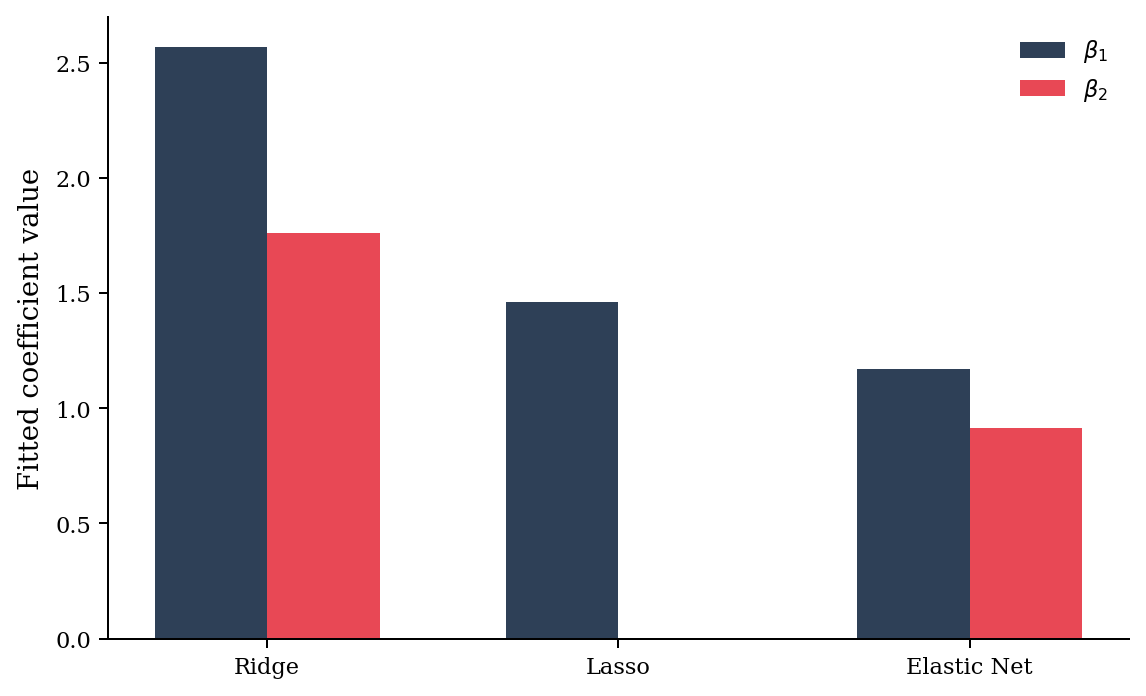
\includegraphics[width=\textwidth, height=0.55\textheight, keepaspectratio]{figures/fig01_elastic_net_grouping.png}
    \end{column}
  \end{columns}
\end{frame}

% Slide 06 — Elastic net: practical guidance
\begin{frame}{Elastic net: practical guidance}
  \begin{itemize}
    \item Default choice when features are correlated \emph{and} you suspect some are irrelevant
    \item Rarely strictly worse than ridge or lasso alone
    \item Cost: one extra hyperparameter --- the blend between $\lambda_1$ and $\lambda_2$ --- tuned via cross-validation
  \end{itemize}
\end{frame}

% Slide 07 — Regularizing deep networks: why it's different
\begin{frame}{Regularizing deep networks: why it's different}
  \begin{itemize}
    \item Deep networks are typically massively overparameterized --- far more weights than training examples
    \item \textbf{Weight decay} is the deep-learning name for L2 regularization, applied inside the optimizer instead of in closed form:
  \end{itemize}
  \[
    w \leftarrow w - \eta\big(\nabla L(w) + \lambda w\big) = (1-\eta\lambda)\,w - \eta\nabla L(w)
  \]
  \begin{itemize}
    \item Every step shrinks $w$ by $(1-\eta\lambda)$ before the gradient update --- the same ridge penalty from Lecture 1, now applied step-by-step rather than solved in closed form (exact for plain gradient descent; adaptive optimizers like Adam decouple this)
    \item Still often not enough alone --- motivates techniques built around \emph{how} networks are trained: early stopping, dropout, data augmentation, batch normalization
  \end{itemize}
\end{frame}

% Slide 08 — Early stopping: the idea
\begin{frame}{Early stopping: the idea}
  \begin{columns}[c]
    \begin{column}{0.46\textwidth}
      \begin{itemize}
        \item Training loss keeps falling with more epochs
        \item Validation loss eventually turns around and rises
        \item Early stopping: halt training at the validation minimum, even though training loss would keep falling
      \end{itemize}
    \end{column}
    \begin{column}{0.5\textwidth}
      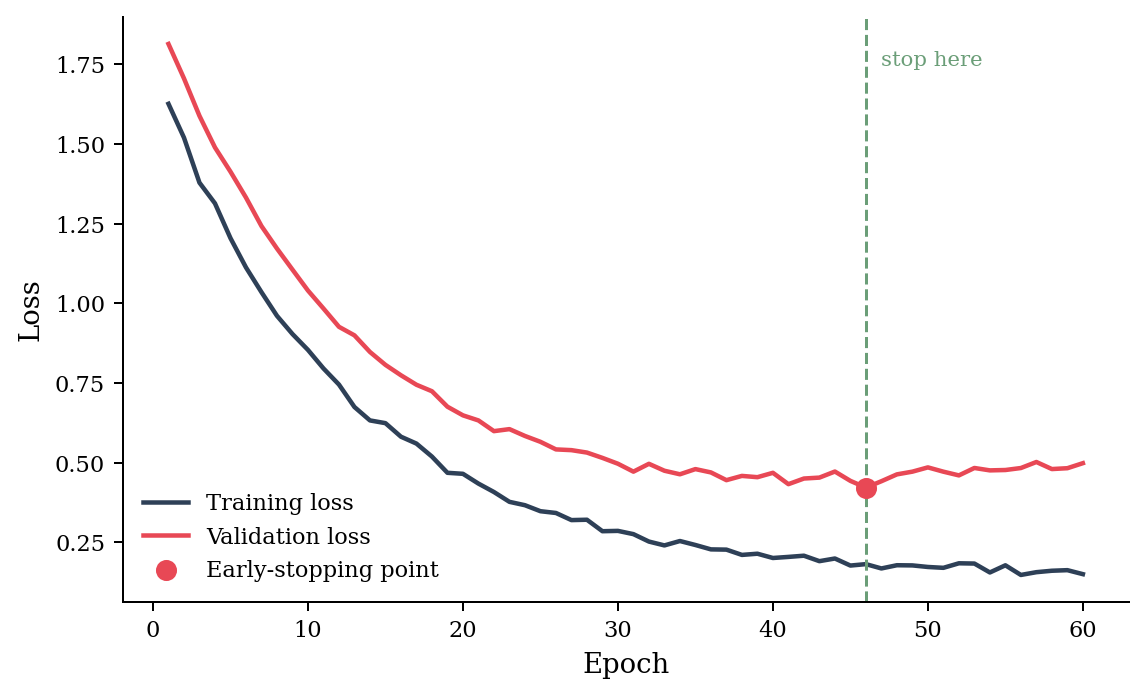
\includegraphics[width=\textwidth, height=0.55\textheight, keepaspectratio]{figures/fig02_early_stopping.png}
    \end{column}
  \end{columns}
\end{frame}

% Slide 09 — Early stopping: why it's a regularizer
\begin{frame}{Early stopping: why it's a regularizer}
  \begin{itemize}
    \item Weights start near initialization and move further away as training progresses
    \item Stopping early caps how far the weights can travel
    \item Informally, this bounds the effective size of the weights --- similar in spirit to an explicit penalty, without adding one
  \end{itemize}
\end{frame}

% Slide 10 — Dropout: the mechanism
\begin{frame}{Dropout: the mechanism}
  \begin{columns}[c]
    \begin{column}{0.42\textwidth}
      \begin{itemize}
        \item At each training step, randomly zero out a fraction of hidden units
        \item A different random subset is dropped every step
        \item Remaining units and their connections train normally
      \end{itemize}
    \end{column}
    \begin{column}{0.54\textwidth}
      \begin{center}
      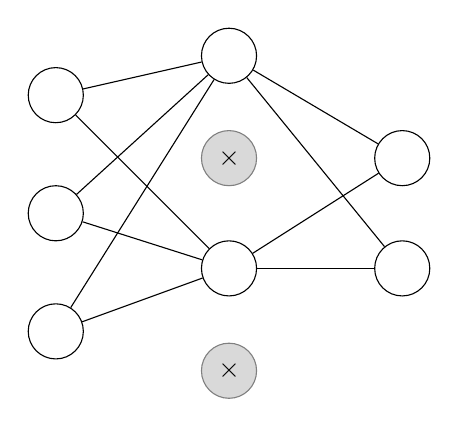
\begin{tikzpicture}[
        neuron/.style={circle, draw, minimum size=7mm},
        dropped/.style={circle, draw=gray, minimum size=7mm, fill=gray!30}
      ]
        % Input layer
        \node[neuron] (i1) at (0, 1.5) {};
        \node[neuron] (i2) at (0, 0) {};
        \node[neuron] (i3) at (0, -1.5) {};
        % Hidden layer (2 of 4 dropped)
        \node[neuron]  (h1) at (2.2, 2.0) {};
        \node[dropped] (h2) at (2.2, 0.7) {$\times$};
        \node[neuron]  (h3) at (2.2, -0.7) {};
        \node[dropped] (h4) at (2.2, -2.0) {$\times$};
        % Output layer
        \node[neuron] (o1) at (4.4, 0.7) {};
        \node[neuron] (o2) at (4.4, -0.7) {};

        % Connections: inputs to active hidden units only
        \draw (i1) -- (h1); \draw (i2) -- (h1); \draw (i3) -- (h1);
        \draw (i1) -- (h3); \draw (i2) -- (h3); \draw (i3) -- (h3);
        % Connections: active hidden units to outputs
        \draw (h1) -- (o1); \draw (h1) -- (o2);
        \draw (h3) -- (o1); \draw (h3) -- (o2);
      \end{tikzpicture}
      \end{center}
    \end{column}
  \end{columns}
\end{frame}

% Slide 11 — Dropout: why it works
\begin{frame}{Dropout: why it works}
  \begin{itemize}
    \item Prevents co-adaptation: no unit can rely on any specific other unit always being present
    \item Approximately equivalent to training and averaging an ensemble of many thinned subnetworks that share weights
    \item Both effects push the network toward more robust, redundant representations
  \end{itemize}
\end{frame}

% Slide 12 — Dropout: train vs. test time
\begin{frame}{Dropout: train vs. test time}
  During training, each unit is kept with probability $p$ and rescaled:
  \[
    \tilde{h} = \frac{1}{p} \cdot m \odot h, \qquad m_i \sim \text{Bernoulli}(p)
  \]
  \begin{itemize}
    \item Rescaling by $1/p$ keeps the expected activation magnitude unchanged
    \item At test time: dropout is turned off entirely, no scaling needed --- this is ``inverted dropout,'' the modern standard
  \end{itemize}
\end{frame}

% Slide 13 — Data augmentation: the idea
\begin{frame}{Data augmentation: the idea}
  \begin{center}
    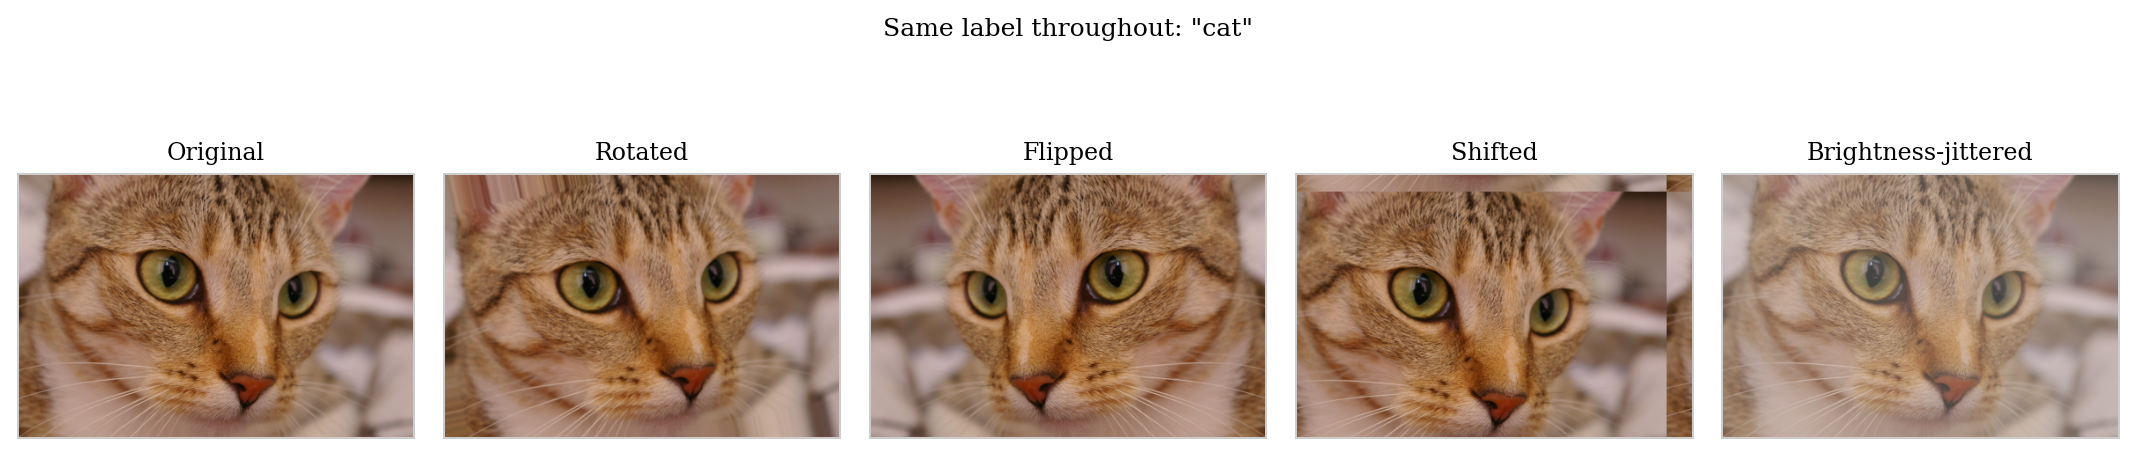
\includegraphics[width=\textwidth, height=0.5\textheight, keepaspectratio]{figures/fig04_data_augmentation.png}
  \end{center}
  Every transformation above is \textbf{label-preserving}: whatever the correct answer was, it still is.
\end{frame}

% Slide 14 — Data augmentation: as regularization
\begin{frame}{Data augmentation: as regularization}
  \begin{itemize}
    \item Augmentation doesn't add new information about the world
    \item It teaches the model which variations \emph{shouldn't} matter for the task
    \item This shrinks the effective hypothesis space toward functions invariant to those transformations
    \item Conceptually similar to constraining the model --- just enforced through the data instead of the loss
  \end{itemize}
\end{frame}

% Slide 15 — Batch normalization: the mechanism
\begin{frame}{Batch normalization: the mechanism}
  For each mini-batch, normalize activations using the batch's own statistics, then apply a learned scale and shift:
  \[
    \hat{x} = \frac{x - \mu_{\text{batch}}}{\sqrt{\sigma^2_{\text{batch}} + \epsilon}}, \qquad y = \gamma \hat{x} + \beta
  \]
  \begin{itemize}
    \item $\mu_{\text{batch}}, \sigma^2_{\text{batch}}$: mean and variance computed from the current mini-batch
    \item $\gamma, \beta$: learned parameters --- the network can undo the normalization if that's optimal
  \end{itemize}
\end{frame}

% Slide 16 — Batch normalization: as implicit regularizer
\begin{frame}{Batch normalization: as implicit regularizer}
  \begin{itemize}
    \item Batch statistics are computed from a randomly sampled mini-batch, not the full dataset
    \item Each example is normalized slightly differently depending on which batch it lands in
    \item This injects a small amount of noise into training --- similar in spirit to dropout
    \item Primary purpose is optimization stability; the regularizing effect is a side benefit
  \end{itemize}
\end{frame}

% Slide 17 — The full toolkit: a comparison table
\begin{frame}{The full toolkit: a comparison table}
  \begin{center}
  \small
  \begin{tabular}{lccc}
    \toprule
    \textbf{Technique} & \textbf{Constrains / perturbs} & \textbf{Extra hyperparameter} & \textbf{Changes training loop?} \\
    \midrule
    Ridge & coefficient L2 norm & $\lambda$ & No \\
    Lasso & coefficient L1 norm & $\lambda$ & No \\
    Elastic net & both norms & $\lambda_1, \lambda_2$ & No \\
    Early stopping & training duration & patience & Yes \\
    Dropout & hidden unit presence & keep prob.\ $p$ & Yes \\
    Data augmentation & input distribution & transform strength & Yes \\
    Batch norm & activation statistics & (usually none)$^*$ & Yes \\
    \bottomrule
  \end{tabular}

  \vspace{6pt}
  {\scriptsize $^*$ $\gamma, \beta$ are learned via backprop like ordinary network weights --- not tuned hyperparameters.}
  \end{center}
\end{frame}

% Slide 18 — Choosing in practice
\begin{frame}{Choosing in practice}
  \begin{itemize}
    \item These techniques are not mutually exclusive --- a typical modern setup combines several at once
    \item Start with weight decay and early stopping: low-cost defaults
    \item Add dropout for large fully-connected layers
    \item Add augmentation whenever label-preserving transformations exist for the data type
    \item Always validate strength/rate choices via cross-validation or a held-out set
  \end{itemize}
\end{frame}

% Slide 19 — Summary & closing
\begin{frame}{Summary \& closing}
  \begin{itemize}
    \item Elastic net closes the classical toolkit: a tunable blend of L1 and L2
    \item Early stopping, dropout, data augmentation, and batch norm regularize deep networks in different ways --- by capping training time, perturbing units, perturbing inputs, or perturbing activation statistics
    \item Every technique here trades a little bias for less variance --- just through a different mechanism
  \end{itemize}
  \vspace{0.5em}
  Now let's put this whole toolkit to work in the lab.
\end{frame}

\end{document}

